% !TEX root = ../thesis.tex
\section{Akustické modelování}
\label{chap:asr:acoustic}

Akustický model představuje v rovnici (\ref{eq:asr:decoding:generic}) podmíněnou pravděpodobnost $p(O|W)$. Úkolem akustického modelu je poskytnout co nejpřesnější odhad této pravděpodobnosti pro libovolnou posloupnost vektorů příznaků $O = \left\{o_1 o_2\ \dots\ o_T\right\}$. Velmi vhodným způsobem modelování řeči se ukázalo být využití tzv. \textbf{skrytých Markovových modelů (HMM)}. Ty vycházejí z principu vytváření řeči člověkem. V průběhu produkce řeči se hlasové ústrojí nachází vždy v krátkém časovém úseku nachází v jednom z konečného počtu konfiguracé. V tomto mikrosegmentu je pak hlasovým ústrojím generovám krátký signál, který zavisí na aktuální konfiguraci. Tento vyprodukovaný zvuk je metodami (popsanými v \ref{chap:asr:parametrization}) převeden na vektor příznaků $O$.

Skrytý Markovův model je model stochastického procesu. Na ten je možné nahlížet jako na pravděpodobnostní konečný automat, který v diskrétních časových okamžicích generuje náhodnou posloupnost vektorů příznaků $O = \left\{o_1 o_2\ \dots\ o_T\right\}$. Model v každém časovém kroku změní stav svůj $s_j$ podle předem daných pravděpodobností přechodu $a_{ij}$. Přechod ze stavu $s_i$ do stavu $s_j$ má za následek vygenerování výstupního vektoru pozorování $o_t$ a to podle rozdělení výstpní pravděpodobnosti $b_j\left(o_t\right)$ příslušné k tomuto stavu \cite{Psutka2006}.

Podmínění pravděpodobnost přechodu $a_{ij}$ určuje, s jakou pravděpodobností přechází model ze stavu $i$ v čase $t$, do stavu $j$ v čase $t+1$. Platí tedy

\begin{equation}
  a_{ij} = p\left(s\left(t+1\right)=s_j|s\left(t\right)=s_i\right),
  \label{eq:asr:acoustic:conditional}
\end{equation}

\noindent kde $s\left(t\right)$ je stav modelu v čase $t$. Další podmínkou je, že pro všechny stavy $i$, $i=1,2,\dots\,N$, platí

\begin{equation}
  \sum_{j=1}^{N} a_{ij} = 1.
  \label{eq:asr:acoustic:state:condition}
\end{equation}

\noindent Funkce rozdělení výstupní pravděpodobnosti $b_j\left(o_t\right)$ popisují rozdělení pravděpodobnosti pozorování $o_t$ produkovaného ve stavu $s_j$ v čase $t$. Pro tuto funkci platí

\begin{equation}
  b_j\left(o_t\right) = P\left(o_t|s\left(t\right)=s\right),
  \label{eq:asr:acoustic:state:output}
\end{equation}

\noindent kde $P$ značí pravděpodobnost, pro kterou u diskrétních rozdělení platí

\begin{equation}
  \sum_o b_j\left(o\right) = 1.
  \label{eq:asr:acoustic:state:output:condition:discrete}
\end{equation}

\noindent Pro spojité rozdělení pak alternativně

\begin{equation}
  \int_o b_j\left(o\right)do = 1.
  \label{eq:asr:acoustic:state:output:condition:continous}
\end{equation}

\noindent V obou případech to platí pro všechny stavy HMM, které mohou generovat výstupní vektor.

Rozdělení výstupní pravděpodobnosti musí být při modelování řečových zvuků dostatečně specifické, aby bylo možné od sebe oddělit různé zvuky, a zároveň dostatečně robustní, aby zahrnulo značnou variabilitu řečového signálu. Toto rozdělení je možné modelovat

\begin{itemize}
  \item spojitým normálním rozdělením se směsí hustotních funkcí,
  \item neuronovými sítěmi.
\end{itemize}

\subsection{Struktura skrytého Markovova modelu}
\label{chap:asr:acoustic:HMM}

Z pohledu rozpoznávání řeči se nejčastěji využívá tzv. levo-pravá struktura Markovova modelu. V průběhu let bylo testováno mnoho různých struktur HMM, např. modely s počtem stavů odvozených od průměrné délky slova pro nějž byl model konstruován, až po pevnou strukturu stavů pro každé slovo. Tyto modely sloužily hlavně pro rozpoznávání izolovaných úseků řeči, nejčastěji slov. V současnosti, kdy je většina systémů konstruovaných pro zpracování souvislé řeči a počet slov ve slovníku může přesahovat 1 milion slov, převažují modely odvozené od menších jednotek, než jsou slova. Takovými jednotkami mohou být například fonémy anebo specifičtější trifóny. Trifón je svým způsobem kontextově závislý foném, který bere v potaz svůj levý a pravý kontext, tj. levý a pravý sousední foném. Přepis slova do fonémově, resp. trifónové struktury, lze ukázat na příkladu izolovaného slova \uv{akcie}, které má přepis \uv{\texttt{sil a k c i j e sil}}, v trifónové podobě je pak zápis následující

\begin{verbatim}
  sil sil-a+k a-k+c k-c+i c-i+j i-j+e j-e+sil sil,
\end{verbatim}

\noindent kde \texttt{sil} má význam pauzy před, případně za vyslovenou promluvou slova \uv{akcie}.

Oproti slovním modelům, u fonémů (monofónů), resp. trifónů, bývá struktura relativně jednoduchá a často je vyjádřena $5$ stavovým modelem (znázorněn na obr. \ref{fig:asr:acoustic:hmm}). Jedná se o $5$ stavový levo-pravý Markovův model, jehož první a poslední stav jsou tzv. neemitující. Jejich primární úlohou je zřetězování jednotlivých HMM modelů trifónů (monofónů) do rozsáhlajších modelů, např. slov, vět ap. Při zřetězení se tyto neemitující stavy vypouštějí. Ostatní stavy modelu jsou emitující a vztahují se k nim odpovídající rozdělení pravděpodobnosti $b_j(.)$.

\begin{figure}[hbpt]
  \centering
  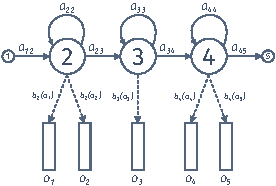
\includegraphics[width=0.7\textwidth]{./ch4-asr/img/hmm_structure.pdf}
  \caption{Příklad levo-pravého Markovova modelu trifónu}
  \label{fig:asr:acoustic:hmm}
\end{figure}

Pokud předpokládáme, že posloupnost slov $W$ je modelována zřetězeným skrytým Markovovým modelem $\lambda$, kde dílčí modely odpovídají fonetickým jednotkám, pak je možné určit pravděpodobnost generování posloupnosti $O$ modelem $\lambda$ jako

\begin{equation}
  P\left(O|\lambda\right) = \sum_{\forall S} P\left(O, S| \lambda\right)P\left(S|\lambda\right) = \sum_{\forall S} a_{s\left(0\right)s\left(1\right)} \prod_{t=1}^{T} b_{s\left(t\right)}\left(o_t\right)a_{s\left(t\right)s\left(t+1\right)},
  \label{eq:asr:acoustic:structure:output}
\end{equation}

\noindent kde posloupnost stavů $S = \left\{s\left(0\right), s\left(1\right),\dots, s\left(T+1\right)\right\}$ je chápána tak, že $s\left(0\right)$ je výstpní a $s\left(T+1\right)$ výstupní neemitující stav modelu $\Theta$ dané promluvy \cite{Psutka2006}. Přitom tento model lze značit trojicí

\begin{equation}
  \lambda = \left[\left\{a_{ij}\right\}_{k,s=1}^{I}; \left\{b_s(.)\right\}_{s=1}^{I};\left\{\pi_{s}\right\}_{s=1}^{I}\right],
  \label{eq:asr:acoustic:structure:marking}
\end{equation}

\noindent kde $a_{ij}$ je přechodová a $b_s(.)$ výstupní pravděpodobnost. Dále $\pi_s$ je rozložení pravděpodobnosti počátečního stavu a $I$ je počet stavů modelu.

Přímé vyčíslení pravděpodobnosti $P\left(O|\lambda\right)$ podle vztahu (\ref{eq:asr:acoustic:state:output}) je z hlediska počtu operací často nerealizovatelné, protože se jedná řádově o $2TN^{T}$ operací násobení. Z tohoto důvodu se proto využívá výpočetně efektivnější tzv. \textbf{algoritmus forward-backward (FB)} s přibližně $N^{2}T$ operací násobení.

Při výpočtu odpředu (forward) se určuje pravděpodobnost $\alpha_j\left(t\right)$ definovaná vztahem

\begin{equation}
  \alpha_{j}\left(t\right) = P\left(o_1o_2\dots o_t, s\left(t\right)=s_j|\lambda\right),
  \label{eq:asr:acoustic:structure:forward}
\end{equation}

\noindent pro výpočet odzadu (backward) se určuje pravděpodobnost $\beta_j\left(t\right)$ definována vztahem


\begin{equation}
  \beta_j\left(t\right) = P\left(o_{t+1}o_{t+2}\dots o_T|s\left(t\right)=s_j|\lambda\right).
  \label{eq:asr:acoustic:structure:backward}
\end{equation}

Podle \cite{Psutka2006} lze snadno dokázat, že výsledná pravděpodobnost $P\left(O|\lambda\right)$ může být vyčíslena vztahem

\begin{equation}
  P\left(O|\lambda\right) = \sum_{s=1}^{N} P\left(O, s\left(t\right) = s | \lambda\right) = \sum_{i = 1}^{N} \alpha_{i}\left(t\right)\beta_{i}\left(t\right)
  \label{eq:asr:acoustic:structure:forward-backward}
\end{equation}

\noindent pro $1 \leq t \leq T$.

\subsection{Trénování parametrů HMM s Gausovkými směsmi}
\label{chap:asr:acoustic:GMM}

Volba struktrury skrytého Markovova modelu je spíše expertní úlohou návrhu. Stanovéní hodnot parametrů modelu je uskutečněno trénováním (odhadem, etimací) na základě trénovacích akustických dat a jejich textových anotací (tzv. korpus). Pro trénování parametrů se využívá tzv. Baum-Welchův interativní algoritmus, což je speciální případ EM algoritmu. Více o něm v \cite{Holmes2001}. Pro odhad střední hodnoty $\mu_{sj}$, tj. složky $m$ gaussovské směsi ve stavu $j$ slouží vztah

\begin{equation}
  \hat{\mu}_{jm} = \frac{\sum_{t=1}^{T}\gamma_{jm}\left(t\right)o_t}{\sum_{t=1}^{T}\gamma_{jm}\left(t\right)},
  \label{eq:asr:acoustic:structure:mu}
\end{equation}

\noindent kde $N$ je počet stavů a $M$ počet složek. Také platí $1 \leq j \leq N$ a $1 \leq m \leq M$. Odhad kovarianční matice $C_{jm}$, tj. složky náležící m-té složce gaussovské směsi ve stavu $j$

\begin{equation}
  \hat{C}_{jm} = \frac{\sum_{t=1}^{T} \gamma_{jm}\left(t\right)\left(o_t - \hat{\mu}_{jm}\right)\left(o_t - \hat{\mu}_{jm}\right)^{T}}{\sum_{t=1}^{T}\gamma_j\left(t\right)},
  \label{eq:asr:acoustic:structure:covariant}
\end{equation}

\noindent kde $1 \leq j \leq N$ a $1 \leq m \leq M$. Odhad váhové složky hustotní směsi $c_{jm}$, tj. složky náležící složce $m$ gaussovské směsi ve stavu $j$ se provádí vztahem

\begin{equation}
  \hat{c}_{jm} = \frac{\sum_{t=1}^{T} \gamma_{jm}\left(t\right)}{\sum_{t=1}^{T}\gamma_j\left(t\right)},
  \label{eq:asr:acoustic:structure:weight}
\end{equation}

\noindent kde $1 \leq j \leq N$ a $1 \leq m \leq M$. Přitom $\gamma_{j}\left(t\right)$ představuje přavděpodobnost, že proces generování posloupnosti $O$ je v čase $t$ ve stavu $j$. Pro vyjádření této pravděpodobnosti $\gamma_{j}\left(t\right)$ platí rovnice (\ref{eq:asr:acoustic:structure:forward-backward}). Pro její definování pak platí vztah

\begin{equation}
 \gamma_{j}\left(t\right) = \frac{P\left(O, s\left(t\right)=j|\lambda\right)}{P\left(O|\lambda\right)} = \frac{\alpha_{j}\left(t\right)\beta_{j}\left(t\right)}{P\left(O|\lambda\right)} ,
  \label{eq:asr:acoustic:structure:gamma}
\end{equation}

\noindent kde $j = 1,\dots,N$ a $t = 1, \dots, T$. Pravděpodobnost, že proces generování posloupnosti $O$ je v čase $t$ ve stavu $j$ a generuje složku $m$ gaussovské hustotní směsi

\begin{equation}
  \gamma_{jm}\left(t\right) = \frac{P\left(O, s\left(t\right)=j, m\left(j,t\right)=m|\lambda\right)}{P\left(O|\lambda\right)} = \frac{\alpha_{j}\left(t\right)\beta_{j}\left(t\right)}{P\left(O|\lambda\right)} \frac{c_{jm}N\left(o_t;\mu_{jm}; C_{jm}\right)}{\sum_{i=1}^{M} c_{ji} N\left(o_t;\mu_{ji};C_{ji}\right) }.
   \label{eq:asr:acoustic:structure:gamma:one}
 \end{equation}

\noindent Akustické modely postavené na kombinaci skrytých Markovových modelů a gaussovských směsí pracují s 10 až 100 tisíc hustotních směsí. Při dimenzi příznakového vektoru (viz \ref{chap:asr:parametrization}) vektoru například $45$ je často nutné provést odhad až 10 miliónů parametrů.

\subsection{Využití neuronových sítí}
\label{chap:asr:acoustic:DNN}

\begin{figure}[hbpt]
  \centering
  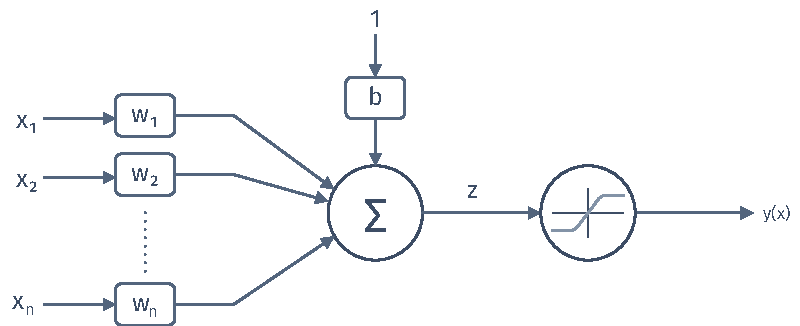
\includegraphics[width=0.7\textwidth]{./ch4-asr/img/neuron.pdf}
  \caption{Schéma perceptronu}
  \label{fig:asr:acoustic:neuron}
\end{figure}

\begin{figure}[hbpt]
  \centering
  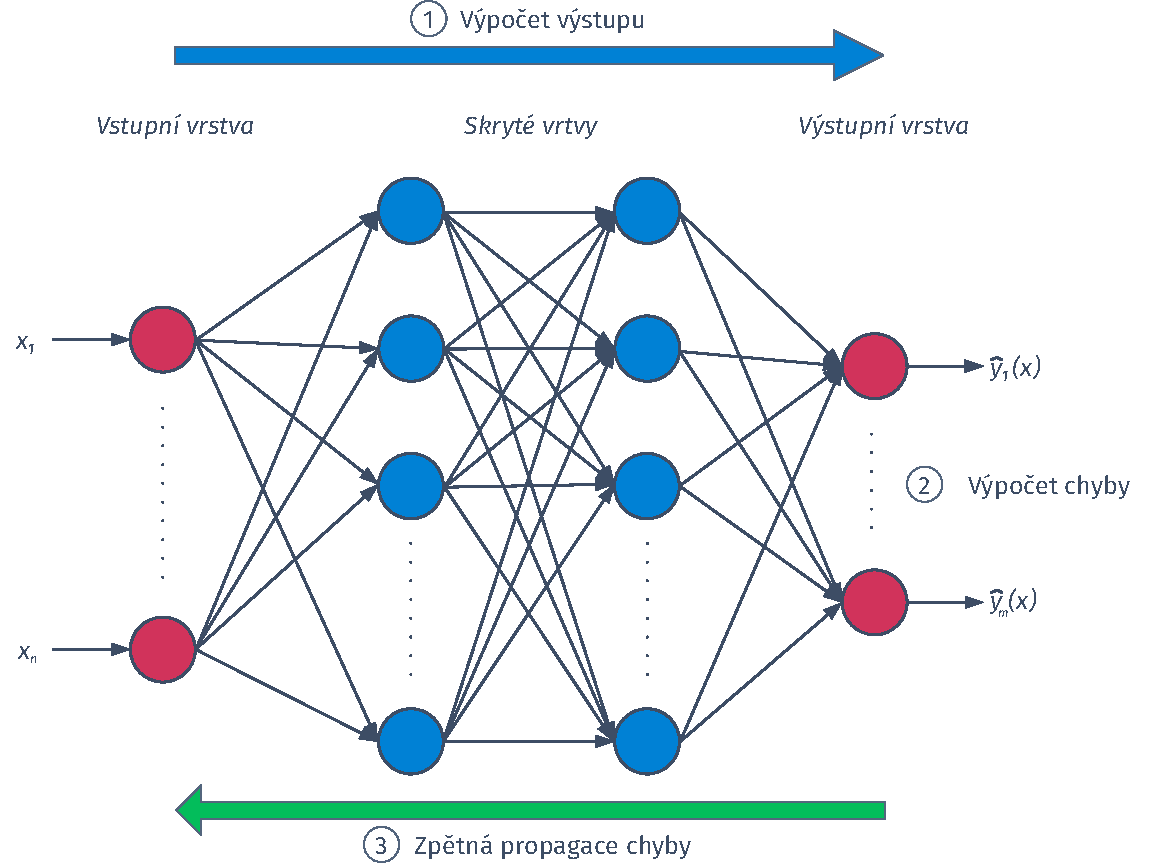
\includegraphics[width=0.9\textwidth]{./ch4-asr/img/dnn-training.pdf}
  \caption{Schéma a princip učení neuronové sítě}
  \label{fig:asr:acoustic:dnn}
\end{figure}
